\documentclass[border=2pt]{standalone}
% Shared TikZ style contract for every schematic figure in this paper.
% Each schematic is a standalone document that \input's this file, so the
% schematics and the matplotlib data figures form one visual system.
%
% Colours are the same Okabe-Ito values as figures/scifig_style.py.

% No font package: the manuscript class sets the body in Computer Modern, so
% the schematics inherit the same family by loading nothing here.
\usepackage{amsmath,amssymb}
\usepackage{tikz}
\usetikzlibrary{arrows.meta,positioning,calc,fit,backgrounds,shapes.geometric,
                shapes.multipart,patterns,decorations.pathreplacing,matrix}

% ---------- Notation shared with the manuscript ----------
% Kept in sync with the definitions in main.tex so that a symbol means the
% same thing in a schematic as it does in the body.
\newcommand{\Cmax}{C_{\max}}
\newcommand{\Zcost}{Z}
\newcommand{\Nb}{\mathcal{N}}

% ---------- Okabe-Ito colour-blind-safe palette ----------
\definecolor{oiblue}{RGB}{0,114,178}
\definecolor{oiorange}{RGB}{230,159,0}
\definecolor{oigreen}{RGB}{0,158,115}
\definecolor{oivermilion}{RGB}{213,94,0}
\definecolor{oipurple}{RGB}{204,121,167}
\definecolor{oisky}{RGB}{86,180,233}
\definecolor{oiyellow}{RGB}{240,228,66}
\definecolor{oigray}{RGB}{110,110,110}

% ---------- Shared node and arrow styles ----------
\tikzset{
  block/.style={draw, rounded corners=2pt, minimum height=6.5mm, minimum width=17mm,
                align=center, font=\footnotesize, fill=oisky!16, line width=0.6pt,
                draw=oiblue!70},
  keyblock/.style={block, fill=oiorange!26, draw=oiorange!85},
  smallblock/.style={block, minimum height=5mm, minimum width=12mm, font=\scriptsize},
  datanode/.style={draw, trapezium, trapezium left angle=70, trapezium right angle=110,
                   align=center, font=\scriptsize, fill=oigreen!14, line width=0.6pt,
                   draw=oigreen!75, inner sep=2pt},
  opnode/.style={draw, circle, inner sep=1pt, minimum size=6mm, font=\scriptsize,
                 fill=oiyellow!45, line width=0.6pt, draw=oigray},
  macnode/.style={draw, rectangle, rounded corners=1pt, minimum size=6mm,
                  font=\scriptsize, fill=oisky!30, line width=0.6pt, draw=oiblue!70},
  modnode/.style={draw, diamond, aspect=1.4, inner sep=1pt, minimum size=6mm,
                  font=\scriptsize, fill=oipurple!28, line width=0.6pt, draw=oipurple!85},
  arrow/.style={-{Stealth[length=2.0mm]}, line width=0.65pt},
  dasharrow/.style={arrow, dashed, draw=oigray},
  thinedge/.style={line width=0.45pt, draw=oigray},
  note/.style={font=\scriptsize, text=oigray, align=center},
  tinynote/.style={font=\tiny, text=oigray, align=center},
  group/.style={draw=oigray, dashed, rounded corners=3pt, inner sep=2.6mm,
                line width=0.5pt},
  grouplabel/.style={font=\scriptsize\itshape, text=oigray},
  whitebg/.style={fill=white, inner sep=1pt},
}

\begin{document}
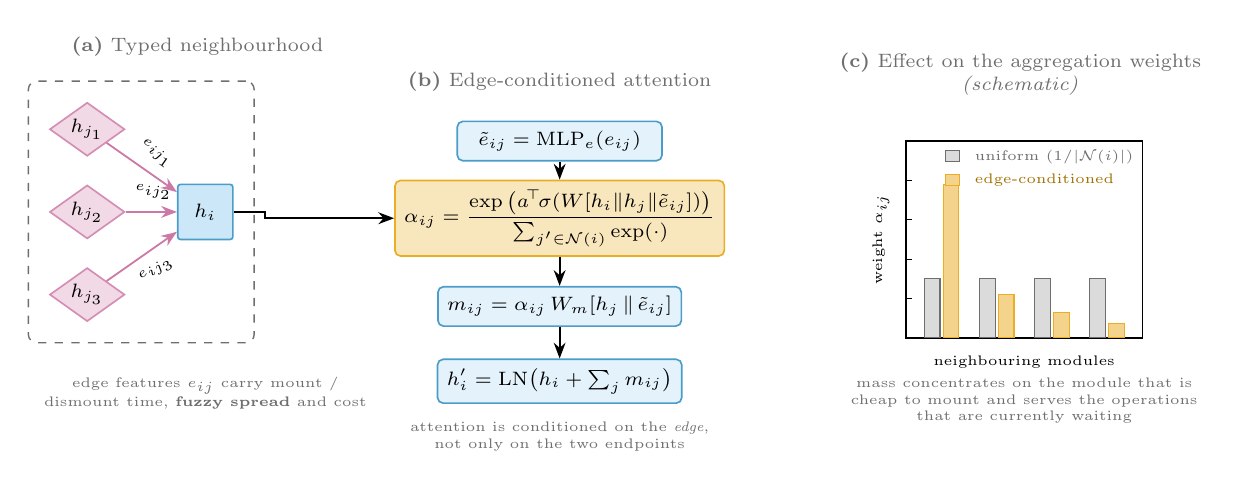
\begin{tikzpicture}

% ================= (a) input: a neighbourhood =================
\node[note] at (-0.1,2.80) {\textbf{(a)} Typed neighbourhood};

\node[macnode, minimum size=7mm] (hi) at (0,0.7) {$h_i$};
\node[modnode, minimum size=6.5mm] (hj1) at (-1.5,1.75) {$h_{j_1}$};
\node[modnode, minimum size=6.5mm] (hj2) at (-1.5,0.7) {$h_{j_2}$};
\node[modnode, minimum size=6.5mm] (hj3) at (-1.5,-0.35) {$h_{j_3}$};

\draw[arrow, draw=oipurple] (hj1) -- node[font=\tiny, above=0.3mm, pos=0.55, sloped] {$e_{ij_1}$} (hi);
\draw[arrow, draw=oipurple] (hj2) -- node[font=\tiny, above=0.3mm, pos=0.55] {$e_{ij_2}$} (hi);
\draw[arrow, draw=oipurple] (hj3) -- node[font=\tiny, below=0.3mm, pos=0.55, sloped] {$e_{ij_3}$} (hi);

\node[tinynote, align=center] at (0,-1.60)
  {edge features $e_{ij}$ carry mount /\\
   dismount time, \textbf{fuzzy spread} and cost};

% ================= (b) the mechanism =================
\node[note] at (4.5,2.35) {\textbf{(b)} Edge-conditioned attention};

\node[smallblock, minimum width=26mm] (emb) at (4.5,1.6)
  {$\tilde{e}_{ij}=\mathrm{MLP}_e(e_{ij})$};
\node[keyblock, minimum width=32mm, minimum height=7mm, font=\scriptsize] (att) at (4.5,0.62)
  {$\alpha_{ij}=\dfrac{\exp\big(a^{\!\top}\!\sigma(W[h_i\|h_j\|\tilde{e}_{ij}])\big)}
    {\sum_{j'\in\mathcal{N}(i)}\exp(\cdot)}$};
\node[smallblock, minimum width=30mm] (msg) at (4.5,-0.5)
  {$m_{ij}=\alpha_{ij}\,W_m[h_j\,\|\,\tilde{e}_{ij}]$};
\node[smallblock, minimum width=30mm] (upd) at (4.5,-1.45)
  {$h_i'=\mathrm{LN}\big(h_i+\textstyle\sum_j m_{ij}\big)$};

\draw[arrow] (emb) -- (att);
\draw[arrow] (att) -- (msg);
\draw[arrow] (msg) -- (upd);
\draw[arrow] (hi.east) -- ++(4mm,0) |- (att.west);

\node[tinynote, align=center] at (4.5,-2.15)
  {attention is conditioned on the \emph{edge},\\not only on the two endpoints};

% ================= (c) effect =================
\node[note] at (10.35,2.45) {\textbf{(c)} Effect on the aggregation weights\\\textit{(schematic)}};

\begin{scope}[shift={(8.9,-0.9)}, x=1.0cm, y=1.0cm]
  % closed rectangular frame, matching the matplotlib figures
  \draw[thinedge, draw=black] (0,0) rectangle (3.0,2.5);
  \foreach \y in {0.5,1.0,1.5,2.0} \draw[thinedge, draw=black] (0,\y) -- (0.08,\y);
  \node[rotate=90, font=\tiny] at (-0.32,1.25) {weight $\alpha_{ij}$};
  \node[font=\tiny] at (1.5,-0.30) {neighbouring modules};

  % uniform aggregation (the ablated variant)
  \foreach \x in {0.45,1.15,1.85,2.55}
    \draw[draw=oigray, fill=oigray!25, line width=0.4pt]
      (\x-0.22,0) rectangle (\x-0.02,0.75);
  % edge-conditioned attention
  \foreach \x/\h in {0.45/1.95, 1.15/0.55, 1.85/0.32, 2.55/0.18}
    \draw[draw=oiorange!85, fill=oiorange!45, line width=0.4pt]
      (\x+0.02,0) rectangle (\x+0.22,\h);

  \node[font=\tiny, text=oigray, anchor=west] at (0.75,2.30) {uniform ($1/|\mathcal{N}(i)|$)};
  \draw[draw=oigray, fill=oigray!25, line width=0.4pt] (0.50,2.24) rectangle (0.68,2.38);
  \node[font=\tiny, text=oiorange!70!black, anchor=west] at (0.75,2.00) {edge-conditioned};
  \draw[draw=oiorange!85, fill=oiorange!45, line width=0.4pt] (0.50,1.94) rectangle (0.68,2.08);
\end{scope}

\node[tinynote, align=center] at (10.4,-1.70)
  {mass concentrates on the module that is\\
   cheap to mount and serves the operations\\
   that are currently waiting};

\begin{scope}[on background layer]
  \node[group, fit=(hj1)(hj3)(hi)] {};
\end{scope}
\end{tikzpicture}
\end{document}
